%-----------------------------------------------------------------------------------------------------
%        روش اجرا.: 2 بار F1 ، 2 بار  F11(به منظور تولید مراجع) ، دوبار Ctrl+Alt+I (به منظور تولید نمایه) و دو بار F1 -------> مشاهده Pdf
%%%%%%%%%%%%%%%%%%%%%%%%%%%%%%%%%%%%%%%%%%%%%%%%%%%%%%
%   TeXstudio as your IDE
%%  برای compile در TeXstudio تنها کافی است منوی Options->Configure TeXstudio را زده و در پنجره Configure TeXstudio در بخش Build گزینه Default Compiler را به XeLaTeX تغییر دهید. سند شما به راحتی compile خواهد شد.
%   F1 & F5 : Build & view
%   F6      : Compile
%   F7      : View
%   --------------
%%%%%%%%%%%%%%%%%%%%%%%%%%%%%%%%%%%%%%%%%%%%%%%%%%%%%%
%        اگر قصد نوشتن رساله دکتری را دارید، در خط زیر به جای msc،
%      کلمه phd را قرار دهید. کلیه تنظیمات لازم، به طور خودکار، اعمال می‌شود.
%%% !TEX TS-program = XeLaTeX
\documentclass[oneside,fleqn,bsc,12pt]{AUTthesis}
%       فایل commands.tex را حتماً به دقت مطالعه کنید؛ چون دستورات مربوط به فراخوانی بسته زی‌پرشین 
%       و دیگر بسته‌ها و ... در این فایل قرار دارد و بهتر است که با نحوه استفاده از آنها آشنا شوید. توجه شود برای نسخه نهایی پایان‌نامه حتماً hyperref را 
%        غیرفعال کنید.

% در این فایل، دستورها و تنظیمات مورد نیاز، آورده شده است.
%-------------------------------------------------------------------------------------------------------------------
% در ورژن جدید زی‌پرشین برای تایپ متن‌های ریاضی، این سه بسته، حتماً باید فراخوانی شود.
\usepackage{amsthm,amssymb,amsmath,amsfonts}
\usepackage[numbers,sort&compress]{natbib}
\usepackage[export]{adjustbox}
\usepackage{xstring}

% بسته‌ای برای تنطیم حاشیه‌های بالا، پایین، چپ و راست صفحه
\usepackage[top=30mm, bottom=30mm, left=25mm, right=30mm]{geometry}
% بسته‌‌ای برای ظاهر شدن شکل‌ها و تصاویر متن
\usepackage{graphicx}
\usepackage{color}
%بسته‌ای برای تنظیم فاصله عمودی خط‌های متن
\usepackage{setspace}
\usepackage{titletoc}
\usepackage{tocloft}
\usepackage[labelsep=space]{caption}
%با فعال کردن بسته زیر فوت‌نوت‌ها در هر صفحه ریست می‌شوند. حالت پیش‌فرض آن ریست شدن در هر فصل می‌باشد.
\usepackage[stable]{footmisc}
\usepackage{enumitem}
%\usepackage{titlesec}
% بسته‌ و دستوراتی برای ایجاد لینک‌های رنگی با امکان جهش
\usepackage[pagebackref=false,colorlinks,linkcolor=blue,citecolor=red]{hyperref}
\usepackage[nameinlink]{cleveref}%capitalize,,noabbrev
 \AtBeginDocument{%
    \crefname{equation}{برابری}{equations}%
    \crefname{chapter}{فصل}{chapters}%
    \crefname{section}{بخش}{sections}%
    \crefname{appendix}{پیوست}{appendices}%
    \crefname{enumi}{مورد}{items}%
    \crefname{footnote}{زیرنویس}{footnotes}%
    \crefname{figure}{شکل}{figures}%
    \crefname{table}{جدول}{tables}%
    \crefname{theorem}{قضیه}{theorems}%
    \crefname{lemma}{لم}{lemmas}%
    \crefname{corollary}{نتیجه}{corollaries}%
    \crefname{proposition}{گزاره}{propositions}%
    \crefname{definition}{تعریف}{definitions}%
    \crefname{result}{نتیجه}{results}%
    \crefname{example}{مثال}{examples}%
    \crefname{remark}{نکته}{remarks}%
    \crefname{note}{یادداشت}{notes}%
}
% چنانچه قصد پرینت گرفتن نوشته خود را دارید، خط بالا را غیرفعال و  از دستور زیر استفاده کنید چون در صورت استفاده از دستور زیر‌‌، 
% لینک‌ها به رنگ سیاه ظاهر خواهند شد که برای پرینت گرفتن، مناسب‌تر است
%\usepackage[pagebackref=false]{hyperref}
% بسته‌ لازم برای تنظیم سربرگ‌ها
\usepackage{fancyhdr}
% بسته‌ای برای ظاهر شدن «مراجع»  در فهرست مطالب
\usepackage[nottoc, notlof, notlot]{tocbibind}
% دستورات مربوط به ایجاد نمایه
\usepackage{makeidx,multicol}
\setlength{\columnsep}{1.5cm}

%%%%%%%%%%%%%%%%%%%%%%%%%%
\usepackage{verbatim}
\makeindex
\usepackage{sectsty}
% فراخوانی بسته زی‌پرشین و تعریف قلم فارسی و انگلیسی
\usepackage{xepersian}%[extrafootnotefeatures]
\ExplSyntaxOn
\cs_set_eq:NN
\etex_iffontchar:D
\tex_iffontchar:D
\cs_undefine:N \c_one
\int_const:Nn \c_one { 1 } 
\ExplSyntaxOff

\SepMark{-}
%حتماً از تک لایو 2014 استفاده کنید.
\settextfont[Scale=1.2]{B Nazanin}
\setlatintextfont{Times New Roman}
\renewcommand{\labelitemi}{$\bullet$}
%%%%%%%%%%%%%%%%%%%%%%%%%%
% چنانچه می‌خواهید اعداد در فرمول‌ها، انگلیسی باشد، خط زیر را غیرفعال کنید.
%در غیر اینصورت حتماً فونت PGaramond را نصب کنید.
% \setdigitfont[Scale=1.1]{XB Yas}%%Yas
%%%%%%%%%%%%%%%%%%%%%%%%%%
% تعریف قلم‌های فارسی اضافی برای استفاده در بعضی از قسمت‌های متن
\defpersianfont\nastaliq[Scale=2]{IranNastaliq}
\defpersianfont\chapternumber[Scale=3]{B Nazanin}
% \chapterfont{\centering}%
%%%%%%%%%%%%%%%%%%%%%%%%%% 
% دستوری برای تغییر نام کلمه «اثبات» به «برهان»
\renewcommand\proofname{\textbf{برهان}}

% دستوری برای تغییر نام کلمه «کتاب‌نامه» به «منابع و مراجع«
\renewcommand{\bibname}{منابع و مراجع}


% Headings for every page of ToC, LoF and Lot
\setlength{\cftbeforetoctitleskip}{-1.2em}
\setlength{\cftbeforelottitleskip}{-1.2em}
\setlength{\cftbeforeloftitleskip}{-1.2em}
\setlength{\cftaftertoctitleskip}{-1em}
\setlength{\cftafterlottitleskip}{-1em}
\setlength{\cftafterloftitleskip}{-1em}
%%\makeatletter
%%%%\renewcommand{\l@chapter}{\@dottedtocline{1}{1em\bfseries}{1em}}
%%%%\renewcommand{\l@section}{\@dottedtocline{2}{2em}{2em}}
%%%%\renewcommand{\l@subsection}{\@dottedtocline{3}{3em}{3em}}
%%%%\renewcommand{\l@subsubsection}{\@dottedtocline{4}{4em}{4em}}
%%%%\makeatother


\newcommand\tocheading{\par عنوان\hfill صفحه \par}
\newcommand\lofheading{\hspace*{.5cm}\figurename\hfill صفحه \par}
\newcommand\lotheading{\hspace*{.5cm}\tablename\hfill صفحه \par}

\renewcommand{\cftchapleader}{\cftdotfill{\cftdotsep}}
\renewcommand{\cfttoctitlefont}{\hspace*{\fill}\LARGE\bfseries}%\Large
\renewcommand{\cftaftertoctitle}{\hspace*{\fill}}
\renewcommand{\cftlottitlefont}{\hspace*{\fill}\LARGE\bfseries}%\Large
\renewcommand{\cftafterlottitle}{\hspace*{\fill}}
\renewcommand{\cftloftitlefont}{\hspace*{\fill}\LARGE\bfseries}
\renewcommand{\cftafterloftitle}{\hspace*{\fill}}

%%%%%%%%%%%%%%%%%%%%%%%%%%
% تعریف و نحوه ظاهر شدن عنوان قضیه‌ها، تعریف‌ها، مثال‌ها و ...
%برای شماره گذاری سه تایی قضیه ها
\theoremstyle{definition}
\newtheorem{definition}{تعریف}[section]
\newtheorem{remark}[definition]{نکته}
\newtheorem{note}[definition]{یادداشت}
\newtheorem{example}[definition]{نمونه}
\newtheorem{question}[definition]{سوال}
\newtheorem{remember}[definition]{یاداوری}
\theoremstyle{theorem}
\newtheorem{theorem}[definition]{قضیه}
\newtheorem{lemma}[definition]{لم}
\newtheorem{proposition}[definition]{گزاره}
\newtheorem{corollary}[definition]{نتیجه}
%%%%%%%%%%%%%%%%%%%%%%%%
%%%%%%%%%%%%%%%%%%%
%%% برای شماره گذاری چهارتایی قضیه ها و ...
%%\newtheorem{definition1}[subsubsection]{تعریف}
%%\newtheorem{theorem1}[subsubsection]{قضیه}
%%\newtheorem{lemma1}[subsubsection]{لم}
%%\newtheorem{proposition1}[subsubsection]{گزاره}
%%\newtheorem{corollary1}[subsubsection]{نتیجه}
%%\newtheorem{remark1}[subsubsection]{نکته}
%%\newtheorem{example1}[subsubsection]{مثال}
%%\newtheorem{question1}[subsubsection]{سوال}

%%%%%%%%%%%%%%%%%%%%%%%%%%%%

% دستورهایی برای سفارشی کردن صفحات اول فصل‌ها
\makeatletter
\newcommand\mycustomraggedright{%
 \if@RTL\raggedleft%
 \else\raggedright%
 \fi}
\def\@makechapterhead#1{%
\thispagestyle{style1}
\vspace*{20\p@}%
{\parindent \z@ \mycustomraggedright
\ifnum \c@secnumdepth >\m@ne
\if@mainmatter

\bfseries{\Huge \@chapapp}\small\space {\chapternumber\thechapter}
\thispagestyle{empty}
\par\nobreak
\vskip 0\p@
\fi
\fi
\interlinepenalty\@M 
\Huge \bfseries #1\par\nobreak
\vskip 120\p@

}

\newpage}
\bidi@patchcmd{\@makechapterhead}{\thechapter}{\tartibi{chapter}}{}{}
\bidi@patchcmd{\chaptermark}{\thechapter}{\tartibi{chapter}}{}{}
\makeatother

\pagestyle{fancy}
\renewcommand{\chaptermark}[1]{\markboth{\chaptername~\tartibi{chapter}: #1}{}}

\fancypagestyle{style1}{
\fancyhf{} 
\fancyfoot[c]{\thepage}
\fancyhead[R]{\leftmark}%
\renewcommand{\headrulewidth}{1.2pt}
}


\fancypagestyle{style2}{
\fancyhf{}
\fancyhead[R]{چکیده}
\fancyfoot[C]{\thepage{}}
\renewcommand{\headrulewidth}{1.2pt}
}

\fancypagestyle{style3}{%
  \fancyhf{}%
  \fancyhead[R]{فهرست نمادها}
  \fancyfoot[C]{\thepage}%
  \renewcommand{\headrulewidth}{1.2pt}%
}

\fancypagestyle{style4}{%
  \fancyhf{}%
  \fancyhead[R]{فهرست جداول}
  \fancyfoot[C]{\thepage}%
  \renewcommand{\headrulewidth}{1.2pt}%
}

\fancypagestyle{style5}{%
  \fancyhf{}%
  \fancyhead[R]{فهرست اشکال}
  \fancyfoot[C]{\thepage}%
  \renewcommand{\headrulewidth}{1.2pt}%
}

\fancypagestyle{style6}{%
  \fancyhf{}%
  \fancyhead[R]{فهرست مطالب}
  \fancyfoot[C]{\thepage}%
  \hypersetup{linkcolor=black, citecolor=black}
  \renewcommand{\headrulewidth}{1.2pt}%
}

\fancypagestyle{style7}{%
  \fancyhf{}%
  \fancyhead[R]{نمایه}
  \fancyfoot[C]{\thepage}%
  \renewcommand{\headrulewidth}{1.2pt}%
}

\fancypagestyle{style8}{%
  \fancyhf{}%
  \fancyhead[R]{منابع و مراجع}
  \fancyfoot[C]{\thepage}%
  \renewcommand{\headrulewidth}{1.2pt}%
}
\fancypagestyle{style9}{%
  \fancyhf{}%
  \fancyhead[R]{واژه‌نامه‌ی فارسی به انگلیسی}
  \fancyfoot[C]{\thepage}%
  \renewcommand{\headrulewidth}{1.2pt}%
}
%


%دستور حذف نام لیست تصاویر و لیست جداول از فهرست مطالب
\newcommand*{\BeginNoToc}{%
  \addtocontents{toc}{%
    \edef\protect\SavedTocDepth{\protect\the\protect\value{tocdepth}}%
  }%
  \addtocontents{toc}{%
    \protect\setcounter{tocdepth}{10}%
  }%
}
\newcommand*{\EndNoToc}{%
  \addtocontents{toc}{%
    \protect\setcounter{tocdepth}{\protect\SavedTocDepth}%
  }%
}
\newcounter{savepage}
\renewcommand{\listfigurename}{فهرست اشکال}
\renewcommand{\listtablename}{فهرست جداول}
%\renewcommand\cftsecleader{\cftdotfill{\cftdotsep}}
%%%%%%%%%%%%%%%%%%%%%%%%%%%%%
%%%%%%%%%%%%%%%%%%%%%%%%%%%%

\begin{document}
\baselineskip=.75cm 
\linespread{1.75}
%% -!TEX root = AUTthesis.tex
% در این فایل، عنوان پایان‌نامه، مشخصات خود، متن تقدیمی‌، ستایش، سپاس‌گزاری و چکیده پایان‌نامه را به فارسی، وارد کنید.
% توجه داشته باشید که جدول حاوی مشخصات پروژه/پایان‌نامه/رساله و همچنین، مشخصات داخل آن، به طور خودکار، درج می‌شود.
%%%%%%%%%%%%%%%%%%%%%%%%%%%%%%%%%%%%
% دانشکده، آموزشکده و یا پژوهشکده  خود را وارد کنید
\faculty{دانشکده مهندسی کامپیوتر}
% گرایش و گروه آموزشی خود را وارد کنید
\department{}
% عنوان پایان‌نامه را وارد کنید
\fatitle{بررسی الگوریتم‌های هوش مصنوعی در پیش‌بینی مصرف انرژی ساختمان‌ها}
% نام استاد(ان) راهنما را وارد کنید
\firstsupervisor{دکتر رضا صفابخش}
% \secondsupervisor{}
% نام استاد(دان) مشاور را وارد کنید. چنانچه استاد مشاور ندارید، دستور پایین را غیرفعال کنید.
%\firstadvisor{نام کامل استاد مشاور}
%\secondadvisor{استاد مشاور دوم}
% نام نویسنده را وارد کنید
\name{فرشید }
% نام خانوادگی نویسنده را وارد کنید
\surname{نوشی}
%%%%%%%%%%%%%%%%%%%%%%%%%%%%%%%%%%
\thesisdate{اردیبهشت ۱۴۰۱}

% چکیده پایان‌نامه را وارد کنید
\fa-abstract{
    پیش‌بینی مصرف انرژی برای ساختمان‌ها ارزش بسیار زیادی در تحقیقات بهره‌وری انرژی و پایداری دارد. مدل‌های پیش‌بینی دقیق انرژی، فواید متعددی در برنامه‌ریزی
     و بهینه‌سازی انرژی ساختمان‌ها و پردیس‌ها دارند. برای ساختمان‌های جدید، 
    که در آن داده‌های ثبت شده گذشته در دسترس نیستند، از روش‌های شبیه‌سازی کامپیوتری برای تجزیه و تحلیل انرژی و پیش‌بینی سناریوهای آینده استفاده می‌شود.
    با این‌ حال برای ساختمان‌های موجود با داده‌های انرژی سری زمانی ثبت‌شده گذشته، تکنیک‌های آماری و یادگیری ماشین دقیق‌تر و سریع‌تر عمل کرده‌اند. 
    این گزارش بررسی‌ای بر الگوریتم‌های هوش مصنوعی موجود برای پیش‌بینی مصرف انرژی سری زمانی انجام داده است.
     اگرچه تاکید بر یک تجزیه‌و‌تحلیل داده‌های سری زمانی منفرد است، اما بررسی فقط به آن محدود نمی‌شود زیرا داده‌های انرژی 
     اغلب با سایر متغیرهای سری زمانی مانند آب‌و‌هوای بیرون و شرایط محیطی داخلی براساس روش محبوب پیش‌بینی که براساس یادگیری ماشین می‌باشد، تجزیه و تحلیل می‌شوند 
      یک بررسی از "مدل ترکیبی"، که ترکیبی از دو یا چند الگوریتم پیش‌بینی است نیز ارائه شده است.
      ترکیبات مختلف مدل ترکیبی موثرترین الگوریتم در پیش‌بینی انرژی سری زمانی برای ساختمان‌ها هستند.
}

% کلمات کلیدی پایان‌نامه را وارد کنید
\keywords{یادگیری ماشین، هوش مصنوعی،‌ پیش‌بینی داده‌های سری زمانی‌، مصرف انرژی ساختمان‌ها‌}



\AUTtitle{a}
%%%%%%%%%%%%%%%%%%%%%%%%%%%%%%%%%%
\vspace*{7cm}
\thispagestyle{empty}
\begin{center}

\end{center}
%% -!TEX root = AUTthesis.tex
% در این فایل، عنوان پایان‌نامه، مشخصات خود، متن تقدیمی‌، ستایش، سپاس‌گزاری و چکیده پایان‌نامه را به فارسی، وارد کنید.
% توجه داشته باشید که جدول حاوی مشخصات پروژه/پایان‌نامه/رساله و همچنین، مشخصات داخل آن، به طور خودکار، درج می‌شود.
%%%%%%%%%%%%%%%%%%%%%%%%%%%%%%%%%%%%
% دانشکده، آموزشکده و یا پژوهشکده  خود را وارد کنید
\faculty{دانشکده مهندسی کامپیوتر}
% گرایش و گروه آموزشی خود را وارد کنید
\department{}
% عنوان پایان‌نامه را وارد کنید
\fatitle{بررسی الگوریتم‌های هوش مصنوعی در پیش‌بینی مصرف انرژی ساختمان‌ها}
% نام استاد(ان) راهنما را وارد کنید
\firstsupervisor{دکتر رضا صفابخش}
% \secondsupervisor{}
% نام استاد(دان) مشاور را وارد کنید. چنانچه استاد مشاور ندارید، دستور پایین را غیرفعال کنید.
%\firstadvisor{نام کامل استاد مشاور}
%\secondadvisor{استاد مشاور دوم}
% نام نویسنده را وارد کنید
\name{فرشید }
% نام خانوادگی نویسنده را وارد کنید
\surname{نوشی}
%%%%%%%%%%%%%%%%%%%%%%%%%%%%%%%%%%
\thesisdate{اردیبهشت ۱۴۰۱}


\AUTtitle{b}
%%%%%%%%%%%%%%%%%%%%%%%%%%%%%%%%%%
% تاییدیه دفاع
%\newpage
\thispagestyle{empty}
%\fontsize{18pt}{19pt}\selectfont

\section*{صفحه فرم ارزیابی و تصویب پایان نامه- فرم تأیید اعضاء كميته دفاع}

\fontsize{12pt}{14pt}\selectfont
%\renewcommand{\baselinestretch}{1.5}
\vspace*{1cm}
   در این صفحه فرم دفاع یا تایید و تصویب پایان نامه موسوم به فرم کمیته دفاع- موجود در پرونده آموزشی- را قرار دهید.
\vspace*{1cm}


\subsection*{نکات مهم:}
 
\begin{itemize}
\item
	نگارش پایان نامه/رساله باید به
	{\color{red}
		زبان فارسی
	}
	و بر اساس آخرین نسخه دستورالعمل و راهنمای تدوین پایان نامه های دانشگاه صنعتی امیرکبیر باشد.(دستورالعمل و راهنمای حاضر)
\item رنگ جلد پایان نامه/رساله چاپي كارشناسي، كارشناسي ارشد و دكترا  بايد به ترتيب مشكي، طوسي و سفيد رنگ باشد.  
\item چاپ و صحافی پایان نامه/رساله بصورت
{\color{red}
	پشت و رو(دورو)
}
بلامانع است و انجام آن توصيه مي شود. 
\end{itemize}
%%%%%%%%%%%%%%%%%%%%%%%%%%%%%%%%%%%%%%%%%%%%%%%%%%%%%%%%%%%%%%%%%%%%%%%%%%%%%%%%%%%%%%%%%%%%%%%%%%
%%%%%%%%%%%%%%%%%%%%%%%%%%%%%%%%%%%%%%%%%%%%%%%%%%%%%%%%%%%%%%%%%%%%%%%%%%%%%%%%%%%%%%%%%%%%%%%%%%
\newpage
\thispagestyle{empty}
\begin{picture}(50,50)
  \put(17,0){
\includegraphics[scale=1.1]{fa-logo}}
  \put(4.5,-13){\footnotesize{دانشگاه صنعتی امیرکبیر}}
  \put(10.5,-27){\footnotesize{(پلی‌تکنیک تهران)}}
  \put(170,30){\bf{به نام خدا}}
  \put(140,-5){\Large\bf{تعهدنامه اصالت اثر}}
  \put(310,0){تاریخ: \datethesis}
\end{picture}

\vspace*{2.5cm}

اينجانب {\bf{\fname\lname}} متعهد می‌شوم که مطالب مندرج در این پایان‌نامه حاصل کار پژوهشی اینجانب تحت نظارت و راهنمایی اساتید دانشگاه صنعتی امیرکبیر بوده و به دستاوردهای دیگران که در این پژوهش از آنها استفاده شده است مطابق مقررات و روال متعارف ارجاع و در فهرست منابع و مآخذ ذکر گردیده است. این پایان‌نامه قبلاً برای احراز هیچ مدرک هم‌سطح یا بالاتر ارائه نگردیده است.

در صورت اثبات تخلف در هر زمان، مدرک تحصیلی صادر شده توسط دانشگاه از درجه اعتبار ساقط بوده و دانشگاه حق پیگیری قانونی خواهد داشت.


کلیه نتایج و حقوق حاصل از این پایان‌نامه متعلق به دانشگاه صنعتی امیرکبیر می‌باشد. هرگونه استفاده از نتایج علمی و عملی، واگذاری اطلاعات به دیگران یا چاپ و تکثیر، نسخه‌برداری، ترجمه و اقتباس از این پایان نامه بدون موافقت کتبی دانشگاه صنعتی امیرکبیر ممنوع است. 
نقل مطالب با ذکر مآخذ بلامانع است.\\
\vspace{2.5cm}


{\centerline {\bf{\fname\lname}}}
\vspace*{.2cm}
{\centerline{امضا}}
%%%%%%%%%%%%%%%%%%%%%%%%%%%%%%%%%
% چنانچه مایل به چاپ صفحات «تقدیم»، «نیایش» و «سپاس‌گزاری» در خروجی نیستید، خط‌های زیر را با گذاشتن ٪  در ابتدای آنها غیرفعال کنید.
% پایان‌نامه خود را تقدیم کنید
% نیایش خود را در فایل زیر بنویسید.
\begin{acknowledgementpage}

\vspace{1.5cm}

{\large\nastaliq
{
{\par \noindent
تقدیم به پدر بزرگوار و مادر مهربانم}
\\[0.1cm]
{\par \noindent
آن دو فرشته‌ای که از خواسته‌هایشان گذشتند، سختی‌ها را به جان خریدند و خود را سپر بلای مشکلات و ناملایمات کردند تا من به جایگاهی که اکنون در آن ایستاده‌ام برسم.
}
}
}

\end{acknowledgementpage}
\newpage
% سپاسگزاری را در فایل زیر بنویسید.
%%%%%%%%%%%%%%%%%%%%%%%%%%%%%%%%%%%%
\newpage\thispagestyle{empty}
% سپاس‌گزاری
{\nastaliq
سپاس‌گزاری
}
\\[2cm]
زندگي صحنه یکتای هنرمندی ماست، هرکسي نغمه خود خواند و از صحنه رود، صحنه پیوسته بجاست، خرم آن نغمه که مردم بسپارند به یاد.
\\
خدا را شاکرم که به من توفیق داد تا بتوانم در راه شناخت جهان پیرامونم تلاش کنم.
\\
از استاد گرامي جناب آقای دکتر رضا صفابخش که درانتخاب و پیشبرد این پروژه به عنوان استاد پروژه، کمکهای فراواني به این جانب داشتند، کمال تشکر را دارم.
\\
همچنین  از  جناب  آقای علیرضا صالحی نژاد در  تهیه  این  گزارش،  به  من  کمک  کردند کمال سپاس را دارم.












% با استفاده از دستور زیر، امضای شما، به طور خودکار، درج می‌شود.
\signature








%%%%%%%%%%%%%%%%%%%%%%%%%%%%%%%%%%%%%%%%%
%%%%%%%%%%%%%%%%%%%%%%%%%%%%%%%%%کدهای زیر را تغییر ندهید.
\newpage\clearpage

\pagestyle{style2}

\vspace*{-1cm}
\section*{\centering چکیده}
%\addcontentsline{toc}{chapter}{چکیده}
\vspace*{.5cm}
\ffa-abstract
\vspace*{2cm}


{\noindent\large\textbf{واژه‌های کلیدی:}}\par
\vspace*{.5cm}
\fkeywords
% دستور زیر برای شماره گذاری صفحات قبل از فصل اول با حروف ابجد است.
\pagenumbering{harfi}
%-----------------------------------------------------------------------------
% فایل زیر دستورات مربوط به نمایش صفحات فهرست مطالب- فهرست اشکال و جداول است.
% {\pagestyle{style2}
% \tableofcontents}\newpage
%
% \listoffigures
\cleardoublepage
\pagestyle{style6}
\tableofcontents
\addtocontents{toc}{\tocheading}% add heading to the first page in ToC, after frontmatter entries
\pagestyle{style6}
\cleardoublepage

%اگر لیست تصاویر و لیست جداول ندارید ، کدهای زیر را با گذاشتن % در ابتدای آنها، غیرفعال کنید.
\BeginNoToc
%============
\addtocontents{lof}{\lofheading}% add heading to the first page in LoF
\pagestyle{style5}
\listoffigures
\thispagestyle{style5}
\cleardoublepage
%============
\addtocontents{lot}{\lotheading}% add heading to the first page in LoT
\thispagestyle{style4}
\listoftables
\thispagestyle{style4}
%============
%\cleardoublepage
%
\cleardoublepage
\setcounter{savepage}{\arabic{page}}
\mainmatter
\EndNoToc
% در صورت تمایل می‌توانید با فعال کردن دستور بالا، لیست تصاویر را به  پایان‌نامه خود اضافه کنید.
%-------------------------------------------------------------------------symbols(فهرست نمادها)
% وجود لیست نمادها الزامیست.(لطفاً نمادهای خود را جایگذین نمادهای پیش‌فرض کنید.)
% %%%%%%%%%%%%%

% {\centering\LARGE\textbf{فهرست نمادها}\par}%

% \pagenumbering{harfi}
% \setcounter{page}{\thesavepage}
% %\setcounter{page}{6}
% \vspace*{1cm}

% \pagestyle{style3}
%\thispagestyle{empty}
%\addcontentsline{toc}{chapter}{فهرست نمادها}
% \symb{\text{ نماد}}{مفهوم}
% \\
% %مقادیر بالا را تغییر ندهید
% %%%%%%%%%%%%%%%%%%%%%%%%%%%%%%%%%%%%%%%%%%%%%%%%%%%%%%%%%
% \symb{\mathbb{R}^n}{
% فضای اقلیدسی با بعد $n$
% }
% \symb{\mathbb{S}^n}{
% کره یکه $n$ بعدی
% }
% \symb{M^m}{
% خمینه $m$-بعدی $M$
% }
% \symb{\mathfrak{X}(M)}{
% جبر میدان‌های  برداری هموار روی $M$
% }
% \symb{\mathfrak{X}^1(M)}{
% مجموعه میدان‌های برداری هموار یکه روی $(M,g)$ 
% }
% \symb{\Omega^p(M)}{
% مجموعه $p$-فرمی‌های روی خمینه $M$
% }
% \symb{Q}{
% اپراتور ریچی
% }
% \symb{\mathcal{R}}{
% تانسور انحنای ریمان
% }
% \symb{ric}{
% تانسور ریچی
% }
% \symb{L}{
% مشتق لی
% }
% \symb{\Phi}{
% 2-فرم اساسی خمینه تماسی
% }
% \symb{\nabla}{
% التصاق لوی-چویتای
% }
% \symb{\Delta}{
% لاپلاسین ناهموار
% }
% \symb{\nabla^*}{
% عملگر خودالحاق صوری القا شده از التصاق لوی-چویتای
% }
% \symb{g_s}{
% متر ساساکی
% }
% \symb{\nabla}{
% التصاق لوی-چویتای وابسته به متر ساساکی
% }
% \symb{\Delta}{
% عملگر لاپلاس-بلترامی روی $p$-فرم‌ها
% }

%%%%%%%%%%%%%%%%%%%%%%%%%%%%%%%%%%%%%%%

% \thispagestyle{style3}
% \newpage
%\pagestyle{style1}
%%%%%%%%%%%%%%%%%%%%%%%%%%%%%%%%%%%%


\pagenumbering{arabic}
\pagestyle{style1}
%--------------------------------------------------------------------------chapters(فصل ها)
\chapter{مقدمه}

آژانس بین‌المللی انرژی، بهره‌وری انرژی در ساختمان‌ها را به عنوان یکی از پنج اقدام برای تضمین کربن‌زدایی طولانی‌ مدت بخش انرژی شناسایی کرده است\cite{DEB2017902}
در کنار مزایای زیست محیطی، بهره‌وری انرژی ساختمان دارای مزایای اقتصادی گسترده ای نیز می‌باشد.
 ساختمان‌هایی با سیستم‌های انرژی کارآمد و استراتژی‌های مدیریتی هزینه‌های عملیاتی بسیار کمتری دارند. اکنون بسیاری از کشورها اجرای قوانین و مقررات انرژی را
 برای انواع ساختمان‌ها تسریع کرده‌اند. این مقررات الزامات اساسی برای دستیابی به یک طراحی کارآمد انرژی برای ساختمان‌های 
 جدید با هدف کاهش مصرف انرژی نهایی و انتشار \lr{CO2} مرتبط را ترسیم می‌کند. 
 علاوه بر این، بسیاری از نرم افزارهای کامپیوتری نیز برای طراحی بهینه انرژی ساختمان‌های جدید توسعه یافته 
 و به طور گسترده پیاده‌سازی شده‌اند. در مورد تکنیک‌های موجود تجزیه و تحلیل انرژی ساختمان
  به کمک کامپیوتر و ابزارهای نرم‌افزاری در \cite{ALHOMOUD2001421, CRAWLEY2008661} اطلاعات دقیقی موجود هستند. این مقررات و ابزارهای کامپیوتری مربوط
   به ساختمان‌های جدید است و در واقع بسیار موثر هستند. با این حال، هنگامی که ساختمان در حال فعالیت است، عوامل زیادی بر رفتار
   انرژی یک ساختمان حاکم هستند، مانند شرایط آب و هوایی، برنامه حضور ساکنین ساختمان، خواص حرارتی مصالح ساختمانی، فعل و انفعالات پیچیده 
  سیستم‌های انرژی مانند گرمایش و تهویه‌هوا و روشنایی و غیره. به دلیل این فعل و انفعالات پیچیده،
   محاسبه دقیق مصرف انرژی از طریق مدل شبیه‌سازی کامپیوتری بسیار دشوار است. به این دلایل، تکنیک‌های داده‌محور برای تجزیه و تحلیل مصرف انرژی ساختمان‌های
   موجود بسیار حیاتی است. این تکنیک‌ها بر داده‌های ثبت‌شده گذشته تکیه دارند و
   تلاش می‌کنند مصرف انرژی را بر اساس الگوهای مصرف انرژی قبلی مدل‌سازی کنند. سایر عوامل مؤثر بر مصرف انرژی را می توان برای بهبود
    دقت چنین مدل‌های سری زمانی استفاده کرد. این تکنیک‌ها که از داده‌های گذشته استفاده می‌کنند،
    اغلب تحت «یادگیری ماشین» قرار می‌گیرند و در دو دهه اخیر به طور فعال در مطالعات پیش‌بینی انرژی ساختمان به کار رفته‌اند

\section[اهمیت بهینه سازی عملکرد ساختمان‌ها]{اهمیت بهینه سازی عملکرد ساختمان‌ها\cite{DEB2017902}}

برای دستیابی به سطح بهینه عملکرد انرژی در ساختمان‌ها، نصب سیستم‌های انرژی کارآمد باید با استراتژی‌های عملیاتی و مدیریتی مناسب دنبال شود. 
این امر مستلزم نظارت و مدیریت مداوم داده‌های انرژی سری زمانی همراه با سایر عوامل موثر بر عملکرد انرژی ساختمان ها است. 
در رابطه با نظارت مستمر و مدیریت مصرف انرژی در ساختمان های موجود، پیش‌بینی نقش بسزایی دارد. می‌تواند مجموعه‌ای از شرایط مرزی و اهداف را برای مدیران و 
مالکان تأسیسات ساختمانی فراهم کند که مصرف انرژی ساختمان به طور ایده‌آل باید در آن قرار گیرد (هدف‌های روزانه، هفتگی، ماهانه و سالانه). 
همانطور که مدل پیش‌بینی سری‌های زمانی از الگوهای مصرف انرژی قبلی یاد می‌گیرد، افزایش تدریجی مقادیر مصرف انرژی پیش‌بینی‌شده
 در یک دوره زمانی ممکن است مدیران تأسیسات را در مورد جنبه‌های تعمیر و نگهداری ساختمان و سیستم‌های انرژی آگاه کند. 
علاوه بر رویکرد پیش‌بینی سری‌های زمانی، سایر رویکردهای سری غیرزمانی را می‌توان برای اهداف بهینه‌سازی ساختمان اتخاذ کرد
 و همچنین می‌توان آنها را با سایر مدل‌های شبیه‌سازی کامپیوتری برای استخراج اشغال و
  سایر عوامل عملیاتی ترکیب کرد.
  \\
   یانگ\LTRfootnote{\lr{Yang}} و همکاران در بهینه سازی انرژی مبتنی بر شبیه سازی برای یک ساختمان آزمایشی در 
  اسپانیا، یک چارچوب بهینه‌سازی الگوریتم ژنتیک موازی
  مبتنی بر وب \LTRfootnote{\lr{GA}} که از منابع محاسباتی توزیع‌شده استفاده می‌کند تا زمان محاسبه
   را کاهش دهد استفاده کردند.پتری \LTRfootnote{\lr{Petri}} و همکاران یک سیستم بهینه‌سازی مبتنی بر مدولار ارائه کردند
    که شبیه‌سازی انرژی و بهینه‌سازی را با استفاده از شبکه عصبی مصنوعی ترکیب می‌کند.
    این برنامه کاهش قابل توجه انرژی (کیلووات ساعت) را در یک سناریوی واقعی نشان داد.
    با این حال، این امر مستلزم تجهیز ساختمان به حسگرها و عملگرها برای نظارت، کنترل
    و بهینه سازی بود. این ممکن است در مورد اکثر زیرساخت های ساختمان موجود نباشد.
    چنین چالش هایی مورد بحث قرار می گیرند. با این حال، همچنین خاطرنشان می شود
    که پتانسیل صرفه جویی انرژی مرتبط در ساختمان ها به راه اندازی، ردیابی عملکرد
    و استراتژی های کنترل پیشرفته مربوط می شوند. این امر به عوامل بسیاری از جمله منابع مالی،
    حمایت از سیاست، آگاهی سبز، مواد سبز و فناوری و غیره وابسته است.
    \\
    زونگ\LTRfootnote{\lr{Zong}} و همکاران در مورد چالش های اجرای یک مدل اقتصادی 
    استراتژی کنترل پیش بینی \LTRfootnote{\lr{EMPC}} برای ساختمان های هوشمند بحث کردند. مشاهده شد که هنوز چالش‌هایی
     در کاربرد کنترل پیش‌بینی مدل از جمله سازش بین ساده‌سازی و پیچیدگی مدل‌سازی 
    دینامیکی حرارتی ساختمان و تعادل بین سیستم‌های چند انرژی وجود دارد.
     هو و همکاران با درک چالش‌ها در ادغام داده‌های عملکرد ساختمان
     با سایر داده‌های مربوط به ساختمان. روش جدیدی را برای پیوند
     دادن داده‌های قطع شده سنتی برای ساخت منابع داده ارائه کرد تا 
    ارزیابی عملکرد ساختمان را به صورت عمیق و روشن‌تر فراهم کند. 
پیش‌بینی سری‌های زمانی برای بهینه‌سازی عملکرد ساختمان ضروری است. هر تکنیک بهینه‌سازی به
 اطلاعاتی در مورد سناریوهای آینده یا یافتن بهترین راه‌حل‌ها در برابر یک معیار
  آزمایشی نیاز دارد. تکنیک های یادگیری ماشین در این زمینه مفید هستند و اغلب در حل این دو مشکل استفاده می شوند. 
با این حال، این بررسی بر جنبه‌های پیش‌بینی سری‌های زمانی بهینه‌سازی ساختمان تمرکز دارد تا اینکه به طور کلی به مسئله بهینه‌سازی نگاه کند. ادغام این دو باید در یک بررسی جداگانه مورد بررسی قرار گیرند.



\section[اهداف بررسی]{اهداف بررسی\cite{DEB2017902}}
مطالعات بررسی اخیر در مورد پیش بینی انرژی، گزارش‌های دقیقی از مدل های پیش بینی موجود و طبقه بندی آنها ارائه می دهد.ژائو \LTRfootnote{\lr{Zhao}} و ماگولس\LTRfootnote{\lr{Magoules}} روش های موجود برای پیش بینی مصرف انرژی ساختمان را در پنج دسته بررسی و طبقه بندی کردند. هیپرت\LTRfootnote{\lr{Hippert}} و همکاران مروری بر پیش بینی بار کوتاه مدت ارائه کرد. سوگانتی\LTRfootnote{\lr{Suganthi}} و ساموئل\LTRfootnote{\lr{Samuel}} مروری بر مدل های تقاضای انرژی برای پیش بینی تقاضا ارائه کردند. فومو\LTRfootnote{\lr{Fumo}} مروری بر برآورد انرژی ساختمان ارائه کرد و همچنین نحوه طبقه بندی مدل های برآورد را مورد مطالعه قرار داد. مارتینز-آلوارز\LTRfootnote{\lr{Martinez-Alvarez}} و همکاران یک نظرسنجی در مورد تکنیک های داده‌کاوی برای پیش بینی سری های زمانی الکتریسیته ارائه کرد. این نظرسنجی بر روی ویژگی های مدل‌ها و پیکربندی آنها متمرکز بود. رضا و خسروی مروری بر تکنیک‌های پیش‌بینی بار کوتاه‌مدت بر اساس تکنیک‌های هوش مصنوعی ارائه کردند. مطالعه اخیر توسط مت داوت\LTRfootnote{\lr{Mat Daut}} و همکاران مروری بر تحلیل پیش‌بینی مصرف انرژی الکتریکی ساختمان با استفاده از روش‌های مرسوم و هوش مصنوعی ارائه کرد. 
همه این بررسی‌ها اطلاعات حیاتی در مورد مدل‌های پیش‌بینی انرژی در مقیاس‌های مختلف ارائه می‌کنند و بر عملکرد برتر مدل‌های ترکیبی تأکید می‌کنند. یک مدل پیش‌بینی می‌تواند مبتنی بر داده‌های استاتیکی باشد که معمولاً یک متغیر وابسته را با مجموعه‌ای از متغیرهای مستقل منطبق می‌کند، یا می‌تواند از داده‌های سری زمانی منفرد یا موازی استفاده کند. 
\\
این مطالعه بر تکنیک های پیش بینی با استفاده از داده های سری زمانی تاکید دارد. اهمیت تجزیه و تحلیل سری های زمانی به دلیل افزایش آگاهی در جمع آوری و پایش داده ها در زمان واقعی است. مصرف انرژی سری زمانی را نیز می توان با داده های سری زمانی شرایط محیطی داخل ساختمان تنظیم کرد. با استقرار حسگرهای بیشتر در ساختمان‌ها و جمع‌آوری داده‌های سری زمانی بیشتر، یک چارچوب مناسب برای تجزیه و تحلیل و شناسایی قابلیت‌های پیش‌بینی مهم است. هدف این بررسی درک تکنیک‌های پیش‌بینی سری‌های زمانی موجود و ارائه مزایا و چالش‌های آن‌ها است. ارزیابی دقیق مدل ترکیبی نیز به دلیل استفاده فزاینده در ادبیات ارائه شده است. از آنجایی که ترکیبات مدل ترکیبی بسیار زیاد است، اینها در بخش بعدی پس از بررسی انتقادی تکنیک‌های اصلی مانند شبکه ی عصبی مصنوعی\LTRfootnote{\lr{artifical neural network}} و میانگین متحرک خودهمبسته یکپارچه\LTRfootnote{\lr{ARIMA}} مورد بررسی انتقادی قرار می‌گیرند. این مقاله مروری همچنین باید مبنایی برای مقایسه کیفی و کمی برای تمام ۶ تکنیک ذکر شده در اینجا فراهم کند. شایان ذکر است که مدل ترکیبی به عنوان یکی از تکنیک های موجود در بین 6 تکنیک ارائه شده در نظر گرفته شده است. در مدل ترکیبی، در مجموع 29 ترکیب وجود دارد که در این بررسی به آنها پرداخته شده است
\\[3em]
\noindent
اهداف این مقاله مروری عبارتند از:
\begin{itemize}
    \item ارائه بررسی‌ای جمعی و جامع از تکنیک‌های اصلی هوش مصنوعی پیش‌بینی سری‌های ‌ز‌‌مانی با توجه به مصرف انرژی ساختمان
    \item انجام یک تحلیل تطبیقی که شامل هر دو جنبه کیفی و کمی این تکنیک‌ها باشد
    \item تشریح ترکیبات مختلف مدل ترکیبی در حین ارزیابی عملکرد و تازگی آن‌ها
\end{itemize}
\begin{figure}[ht!]
    \begin{center}
        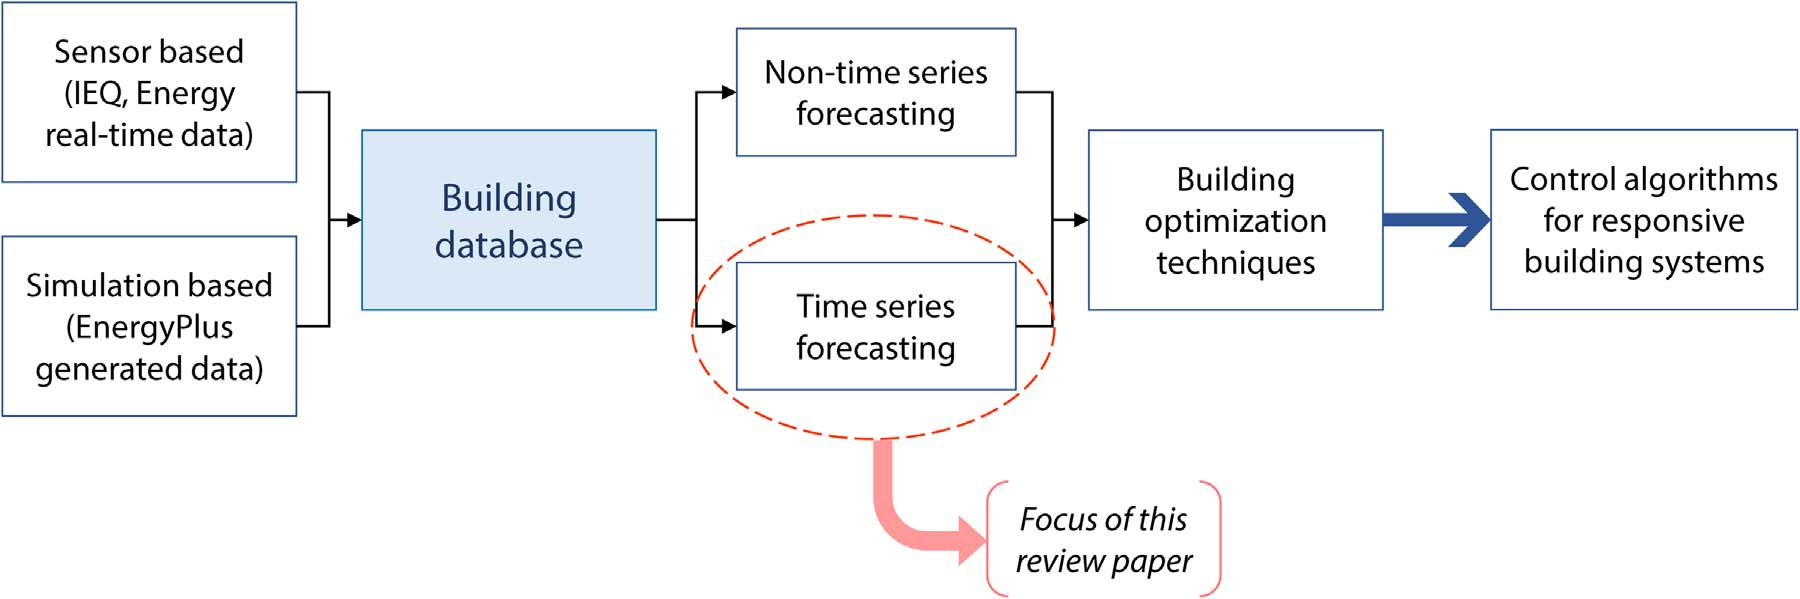
\includegraphics[width=14cm]{images/illustration.jpg}
    \end{center}
    \caption[‌اهمیت پیش‌بینی انرژی ساختمان‌ها برای بهینه سازی ساختمان‌ها]{تمرکز این گزارش نوشتاری در حوزه بهینه‌سازی ساختمان
     \cite{DEB2017902}}
    \label{fig:dc}
    \end{figure}

\noindent
در فصل‌های بعدی نخست توضیحاتی در مورد پیش‌بینی مصرف انرژی ساختمان‌ها میدهیم و در مورد روش‌های تاریخی و قدیمی‌تر از 
الگوریتم‌های هوش‌ مصنوعی صحبت خواهیم کرد که روش‌های مهندسی و آماری را شامل میشوند. در فصل ۳ الگوریتم‌های متنوع هوش مصنوعی برای پیش‌بینی سری داده‌های زمانی معرفی و به طور مفصل شرح داده میشوند و هر یک 
معادلات مورد نیازشان توضیح داده میشود. در فصل ۴ معیار‌های سنجش بین این الگوریتم‌ها معرفی می‌شوند و آزمایش‌های متنوع 
برای یافتن الگوریتم‌های مناسب را گزارش می‌دهیم و در نهایت در فصل ۵ با نتیجه‌گیری از مطالب گفته شده سعی در نتیجه‌گیری گزارش و ارائه پیشنهادات مناسب شده است.
\chapter{الگوریتم های هوش مصنوعی مورد بررسی}
\section{شبکه های عصبی مصنوعی}
\section{ماشین بردار پشتیبان}
\section{میانگین متحرک خودهمبسته یکپارچه}
\section{سری زمانی فازی}
\section{استدلال مبتنی بر مورد}
\section{خلاصه}
\chapter{نتایج تجربی بر روی مجموعه های داده}
%\thispagestyle{empty}

\section{معرفی مجموعه های داده}

\section{مقایسه ی روش های مورد بررسی}
\section{انتخاب بهینه ترین روش پیشنهادی}
\section{خلاصه}

\chapter{جمع‌بندي و نتيجه‌گيري و پیشنهادات}
%%%%%%%%%%%%%%%%%%%%%%%%%%%%%%%%%%%%%%%%%%%
در پايان گزارش‌هاي علمي و فني لازم است كه جمع‌بندي يا نتيجه‌گيري نهايي ارائه شود. در اين موارد مي‌توان آخرين فصل پایان نامه كه پیش از مراجع قرار مي‌گيرد را به اين امر اختصاص داد.
\section{پیشنهادات}
در این بخش پیشنهاداتی که محقق جهت ادامه تحقیقات دارد ارایه می‌گردد. دقت شود که پیشنهادات باید از  تحقیق انجام شده و نتایج ان حاصل شده باشد و از ذکر جملات کلی باید پرهیز کرد.




\chapter{نتيجه‌گيري و پیشنهادها}
%%%%%%%%%%%%%%%%%%%%%%%%%%%%%%%%%%%%%%%%%%%
در بخش پایانی گزارش، جمعبندي و مروري بر سیر مطالب عنوان شده در گزارش خواهیم داشت. همچنین نتایج حاصل را بیان
کرده و پیشنهادهایی براي ادامه کار در این موضوع ارائه میدهیم.
\section{نتیجه‌گیری}
این گزارش ۶ الگوریتم‌ برای پیش‌بینی مصرف انرژی ساختمان‌ها را مورد بررسی قرار داد که برای این الگوریتم‌ها داده‌های مصرف آینده‌ی ساختمان‌ها و مصرف گذشته‌شان موجود بود. 
همچنین در این مقاله اهمیت برخی متغیرها مانند وضعیت دمای محیط و تعداد ساکنین ساختمان در هر زمان نیز مورد توجه قرار گرفتند و اهمیت آن‌ها در تصمیم گیری مشخص گردید.
چندین مدل یادگیری ماشین موفق با استفاده از داده‌های انرژی ثبت‌شده گذشته برای پیش‌بینی کوتاه‌مدت، میان‌مدت و بلندمدت توسعه یافته‌اند. مشاهده می شود 
که هر یک از تکنیک های توصیف شده دارای مجموعه ای از مزایا و معایب است. اینها با توجه به تجزیه و تحلیل داده های انرژی ساختمان به تفصیل تجزیه و تحلیل و ارائه شده اند.
 تأکید ویژه بر مدل ترکیبی داده شده است، که ترکیبی از دو یا چند تکنیک یادگیری ماشینی است به نحوی که هر مدل قدرت دیگری 
 را تحسین می کند. به عنوان مثال، یک مدل ترکیبی که میانگین متحرک خودهمبسته یکپارچه و الگوریتم‌های تکاملی را در نظر می‌گیرد، می‌تواند
  از مدل میانگین متحرک خودهمبسته یکپارچه برای تعیین تناوب و خطی بودن استفاده کند، در حالی که الگوریتم‌ تکاملی می‌تواند به طور موثر باقیمانده‌ها را تعیین کند. ترکیبات مختلفی از مدل ترکیبی و تازگی آنها در
   ادبیات شناسایی شده و به طور سیستماتیک در این مقاله ارائه شده است. مشاهده می‌شود
   که ترکیب تکنیک‌های پیش‌بینی سری‌های زمانی مانند شبکه ی عصبی مصنوعی، میانگین متحرک خودهمبسته یکپارچه به خوبی با 
   تکنیک‌های بهینه‌سازی ترکیب می‌شوند. چنین ترکیب‌هایی به طور گسترده در تحقیقات اختصاص یافته به بهینه‌سازی ساختمان مورد بررسی قرار گرفته‌اند.
    انتظار می رود روند رو به رشد
    در تحقیقات در بهره وری انرژی ساختمان در پرتو انگیزه پایداری جهانی ادامه یابد. این امر نظارت و پیش بینی داده های انرژی در 
    زمان واقعی را در این زمینه مرتبط و حیاتی می کند. این مقاله خلاصه‌ای جامع از تکنیک‌های پیش‌بینی موجود همراه با ترکیبی
     از مدل ترکیبی ارائه می‌کند و راه را برای تحقیقات آینده در زمینه مصرف انرژی ساختمان هموار می‌کند.
     \\
     حوزه بهینه سازی ساختمان بر اساس یک شبکه گسترده جمع آوری داده، نظارت، پیش بینی، بهینه سازی و کنترل است. تمام این زیرساخت‌ها
      همواره به کل هزینه عملیاتی ساختمان می‌افزایند. چالش در اینجا بررسی مزایای اضافه شده از نظر هزینه سرمایه گذاری و هزینه به دست آمده
      به دلیل صرفه جویی در انرژی ناشی از بهینه سازی ساختمان است. مطالعات کمی وجود دارد که بخش مالی را برای کنترل عملکرد و بهینه سازی ساختمان 
     برجسته می کند. این محدودیت در به اشتراک گذاری داده های هزینه یا به دلیل 
     نیروهای بازار درگیر است یا به دلیل محرمانه بودن ماهیت داده های درگیر. لبی الدان\LTRfootnote{Labeodan} 
     و همکاران. کاربردهای شبکه حسگرها و محرک‌های بی‌سیم کم‌هزینه را برای مدل‌سازی اشغال و کنترل روشنایی در یک ساختمان
      اداری مورد بحث قرار داد \cite{labeodan2016application}. هزینه کل سیستم تقریباً 2575 یورو برای 12 ایستگاه کاری بود که
      شامل حسگرهای حرکتی بی سیم و سنسورهای صندلی بود. نتایج نشان می دهد که به طور متوسط 24\% کاهش در مصرف انرژی روشنایی برای یک دوره
      دو هفته ای با هزینه اجرا شده در حدود 215 یورو برای هر ایستگاه کاری است. نویسندگان خاطرنشان کردند که هزینه اولیه بالاتر و عدم آگاهی از عوامل مؤثر
      در کاهش سرعت استقرار حسگرها هستند. با این حال، صرفه جویی در انرژی به دست آمده، سهولت استقرار و بهبود سنجش محیطی این
      را به عنوان یک راه حل مناسب برای دستیابی به عملکرد بهبود 
      یافته ساختمان نشان می دهد. کومار و همکاران همچنین متوجه شد که هزینه سنسورهای نظارت کنترل کیفیت هوای داخلی الزامات استقرار در مقیاس بزرگ برای کنترل و اتوماسیون را
       برآورده نمی کند \cite{kumar2016real}. لیلیس و همکاران اشاره کنید
       که علاقه به راه‌حل‌های 
      مبتنی بر اینترنت اشیا\LTRfootnote{Internet Of Things (IOT)} مدرن برای بهینه‌سازی ساختمان به دلیل عدم برآورد منافع هزینه، مهار شده است \cite{lilis2017towards}. چن و همکاران اشاره کرد
       که هزینه مربوط به مصرف انرژی مجموعه تصادفی ساختمان‌ها در چین با سیستم های اتوماسیون ساختمان تقریباً دو برابر ساختمان های
       بدون سیستم اتوماسیون ساختمان است \cite{chen2016cost}. این به دلیل نقص سنسور و نقص استراتژی کنترل است که منجر به افزایش قابل توجهی در مصرف انرژی نهایی می شود.
        \\
        چند مطالعه مروری شبکه حسگر بی سیم را پوشش داده است که سیستم مدیریت انرژی ساختمان را برای کاربردهای خانه/ساختمان 
        هوشمند فعال کرده است \cite{kazmi2014review,kuzlu2015review}. از آنجایی که فناوری کنترل پیش‌بینی مدل هنوز در مرحله توسعه است و 
        نیاز به بهینه‌سازی سنگین بر اساس نوع و عملکرد ساختمان دارد،
         پیاده‌سازی در حال حاضر بیشتر بر روی بستر آزمایشی و اعتبارسنجی تمرکز دارد. در عین حال، این فناوری هنوز
         با هزینه لازم برای استقرار در مقیاس های بزرگ در دسترس نیست. 
         این چالش ها منجر به نفوذ آهسته اتوماسیون ساختمان و بهینه سازی در کل می شود. دامنه این مقاله مروری، با این حال
        ، محدود به مطالعه تکنیک‌های پیش‌بینی سری‌های زمانی برای مصرف انرژی ساختمان است که بخشی جدایی‌ناپذیر
         از فرآیند بهینه‌سازی و کنترل ساختمان است.
\section{پیشنهادها}
    به طور کلی الگوریتم‌های هوش‌ مصنوعی که در زمینه‌ی پیش‌بینی سری داده‌های زمانی کار میکنند و بخش عمده‌ی آن‌ها که الگوریتم‌های یادگیری ماشین می‌شوند مشکلات و سختی‌های مخصوصی دارند
    از جمله محدودیت‌های مربوط به یادگیری‌آن‌ها که نیازمند داده‌های بسیتر زیاد برای یادگیری و آموزش میباشد و هم‌چنین نیاز به توان پردازشی بالای آن‌ها که از جمله مشکلات روش‌های هوش مصنوعی 
    به طور کلی میباشد. 
    برای حل این مشکل پیشنهاد میشود که الگوریتم‌های نوینی با استفاده از روش‌های ترکیبی توسعه داده بشوند که نیاز به داده‌های زیاد برای یادگیری در آن‌ها کمتر باشد و بتوانند با شبیه‌سازی 
    آموزش ببینند و همچنین برای حل مشکل پردازش‌های سنگین با تحقیقات جدید به سمت برخط کردن یادگیری الگوریتم‌های هوش مصنوعی حرکت بکنیم به این صورت که تمام پردازش‌های مورد نیاز 
    الگوریتممان برروی سرورهای قدرتمندی در سطح منطقه انجام بشوند و ساختمان‌ها مشکل پردازشی‌شان از این نظر مرتفع بشود و تنها برای انجام اندازه‌ی مشخصی از پردازش برروی شبکه ی قدرتمندمان 
    هزینه پرداخت کنند تا هزینه‌هایشان کاهش پیدا بکند.

%--------------------------------------------------------------------------appendix( مراجع و پیوست ها)
\chapterfont{\vspace*{-2em}\centering\LARGE}%

\appendix
\bibliographystyle{unsrt-fa}
\bibliography{references}
% \chapter*{‌پیوست}
\markboth{پیوست}{}
\addcontentsline{toc}{chapter}{پیوست}
موضوعات مرتبط با متن گزارش پایان نامه كه در يكی از گروه‌های زير قرار می‌گيرد، در بخش پيوست‌ها آورده شوند:
\begin{enumerate}
\item  اثبات های رياضی يا عمليات رياضی طولانی‌.‌
\item داده و اطلاعات نمونه (های) مورد مطالعه (\lr{Case Study}) چنانچه طولانی باشد‌.‌
\item نتايج كارهای ديگران چنانچه نياز به تفصيل باشد‌.‌
\item مجموعه تعاريف متغيرها و پارامترها، چنانچه طولانی بوده و در متن به انجام نرسيده باشد‌.‌
\end{enumerate}
% براي شماره‌گذاري روابط، جداول و اشكال موجود در پيوست‌ از ساختار متفاوتي نسبت به متن اصلي استفاده مي‌شود كه در زير به‌عنوان نمونه نمايش داده شده‌است. 
% \begin{equation}
%F=ma
%\end{equation}
\section*{کد میپل }
\begin{latin}
\begin{verbatim}

with(DifferentialGeometry):
with(Tensor):
DGsetup([x, y, z], M)
																	frame name: M
a := evalDG(D_x)
																	D_x
b := evalDG(-2 y z D_x+2 x D_y/z^3-D_z/z^2)


\end{verbatim}
\end{latin}
%--------------------------------------------------------------------------dictionary(واژه نامه ها)
%اگر مایل به داشتن صفحه واژه‌نامه نیستید، خط زیر را غیر فعال کنید.
% \parindent=0pt
% %
\chapter*{واژه‌نامه‌ی فارسی به انگلیسی}
\pagestyle{style9}

\addcontentsline{toc}{chapter}{واژه‌نامه‌ی فارسی به انگلیسی}
%%%%%%
\begin{multicols*}{2}

{\bf آ}
\vspace*{3mm}


\farsiTOenglish{اسکالر}{Scalar}


\vspace*{3mm}
{\bf ب}
\vspace*{3mm}

\farsiTOenglish{بالابر}{Lift}


\vspace*{3mm}
{\bf پ}
%%\vspace*{3mm}

\farsiTOenglish{پایا}{Invariant}



\vspace*{3mm}
{\bf ت}
%%\vspace*{3mm}

\farsiTOenglish{ تناظر }{Correspondence}


\vspace*{3mm}
{\bf ث}
%%\vspace*{3mm}

\farsiTOenglish{ثابت‌ساز}{Stabilizer}

\vspace*{3mm}
{\bf ج}
%%\vspace*{3mm}

\farsiTOenglish{جایگشت}{Permutation}



\vspace*{3mm}
{\bf چ}
%%\vspace*{3mm}


\farsiTOenglish{چند جمله‌ای }{Polynomial}

\vspace*{3mm}
{\bf ح}
%%\vspace*{3mm}

\farsiTOenglish{حاصل‌ضرب دکارتی}{Cartesian product}


\vspace*{3mm}
{\bf خ}
%%\vspace*{3mm}

\farsiTOenglish{خودریختی}{Automorphism}

\vspace*{3mm}
{\bf د}
%%\vspace*{3mm}

\farsiTOenglish{درجه}{Degree}


\vspace*{3mm}
{\bf ر}
%%\vspace*{3mm}


\farsiTOenglish{ریزپردازنده}{microprocessor}


\vspace*{3mm}
{\bf ز}
%%\vspace*{3mm}


\farsiTOenglish{زیرمدول}{Submodule}


\vspace*{3mm}
{\bf س}
%%\vspace*{3mm}

\farsiTOenglish{سرشت}{Character}


\vspace*{3mm}
{\bf ص}
%%\vspace*{3mm}

\farsiTOenglish{صادقانه}{Faithful}

\vspace*{3mm}
{\bf ض}
%%\vspace*{3mm}

\farsiTOenglish{ضرب داخلی}{Inner product}

\vspace*{3mm}
{\bf ط}
%%\vspace*{3mm}


\farsiTOenglish{طوقه}{Loop}


\vspace*{3mm}
{\bf ظ}
%%\vspace*{3mm}


\farsiTOenglish{ظرفیت}{Valency}
 
\vspace*{3mm}
{\bf ع}
%%\vspace*{3mm}


\farsiTOenglish{عدم مجاورت}{Nonadjacency}



\vspace*{3mm}
{\bf ف}
%%\vspace*{3mm}

\farsiTOenglish{فضای برداری}{Vector space}



\vspace*{3mm}
{\bf ک}
%%\vspace*{3mm}

\farsiTOenglish{کاملاً تحویل‌پذیر}{Complete reducibility}


\vspace*{3mm}
{\bf گ}
%%\vspace*{3mm}


\farsiTOenglish{گراف}{Graph}



\vspace*{3mm}
{\bf م}
%%\vspace*{3mm}

\farsiTOenglish{ماتریس جایگشتی}{Permutation matrix }


\vspace*{3mm}
{\bf ن}
%%\vspace*{3mm}

\farsiTOenglish{ناهمبند}{Disconnected}


\vspace*{3mm}
{\bf و}
%%\vspace*{3mm}

\farsiTOenglish{وارون‌پذیر}{Invertible}


\vspace*{3mm}
{\bf ه}
%%\vspace*{3mm}

\farsiTOenglish{همبند}{Connected}



\vspace*{3mm}
{\bf ی}
%%\vspace*{3mm}

\farsiTOenglish{یال}{Edge}




\end{multicols*}
% %%%%%%
\chapter*{ واژه‌نامه‌ی انگلیسی به فارسی}
\pagestyle{style9}
\lhead{\thepage}\rhead{واژه‌نامه‌ی انگلیسی به فارسی}
\addcontentsline{toc}{chapter}{واژه‌نامه‌ی انگلیسی به فارسی}

\LTRmulticolcolumns
\begin{multicols}{2}
{\hfill\bf  \lr{A}}
%%\vspace*{1.5mm}

\englishTOfarsi{Automorphism}{خودریختی}

\vspace*{3mm}
{\hfill\bf   \lr{B}}
%%\vspace*{1.5mm}

\englishTOfarsi{Bijection}{دوسویی}

\vspace*{3mm}
{\hfill\bf   \lr{C}}
%%\vspace*{1.5mm}

\englishTOfarsi{Cycle group}{گروه دوری}

\vspace*{3mm}
{\hfill\bf   \lr{D}}
%%\vspace*{1.5mm}

\englishTOfarsi{Degree}{درجه}

\vspace*{3mm}
{\hfill\bf   \lr{E}}
%%\vspace*{1.5mm}

\englishTOfarsi{Edge}{یال}

\vspace*{3mm}
{\hfill\bf   \lr{F}}
%%\vspace*{1.5mm}

\englishTOfarsi{Function}{تابع}

\vspace*{3mm}
{\hfill\bf   \lr{G}}
%%\vspace*{1.5mm}

\englishTOfarsi{Group}{گروه}

\vspace*{3mm}
{\hfill\bf   \lr{H}}
%%\vspace*{1.5mm}

\englishTOfarsi{Homomorphism}{همریختی}

\vspace*{3mm}
{\hfill\bf   \lr{I}}
%%\vspace*{1.5mm}

\englishTOfarsi{Invariant}{پایا}

\vspace*{3mm}
{\hfill\bf   \lr{L}}
%%\vspace*{1.5mm}

\englishTOfarsi{Lift}{بالابر}

\vspace*{3mm}
{\hfill\bf   \lr{M}}
%%\vspace*{1.5mm}

\englishTOfarsi{Module}{مدول}

\vspace*{3mm}
{\hfill\bf   \lr{N}}
%%\vspace*{1.5mm}

\englishTOfarsi{Natural map}{نگاشت طبیعی}

\vspace*{3mm}
{\hfill\bf   \lr{O}}
%%\vspace*{1.5mm}

\englishTOfarsi{One to One}{یک به یک}

\vspace*{3mm}
{\hfill\bf   \lr{P}}
%%\vspace*{1.5mm}

\englishTOfarsi{Permutation group}{گروه جایگشتی}

\vspace*{3mm}
{\hfill\bf   \lr{Q}}
%%\vspace*{1.5mm}

\englishTOfarsi{Quotient graph}{گراف خارج‌قسمتی}

 \vspace*{3mm}
{\hfill\bf   \lr{R}}
%%\vspace*{1.5mm}

\englishTOfarsi{Reducible}{تحویل پذیر}

\vspace*{3mm}
{\hfill\bf   \lr{S}}
%%\vspace*{1.5mm}

\englishTOfarsi{Sequence}{دنباله}

 \vspace*{3mm}
{\hfill\bf   \lr{T}}
%%\vspace*{1.5mm}

\englishTOfarsi{Trivial character}{سرشت بدیهی}

\vspace*{3mm}
{\hfill\bf   \lr{U}}
%%\vspace*{1.5mm}

\englishTOfarsi{Unique}{منحصربفرد}

\vspace*{3mm}
{\hfill\bf   \lr{V}}
%%\vspace*{1.5mm}

\englishTOfarsi{Vector space}{فضای برداری}
\end{multicols}
%--------------------------------------------------------------------------index(نمایه)
%اگر مایل به داشتن صفحه نمایه نیستید، خط زیر را غیر فعال کنید.
% \pagestyle{style7}
% \printindex
% \pagestyle{style7}
% %کلمات کلیدی انگلیسی
\latinkeywords{Write a 3 to 5 KeyWords is essential. Example: AUT, M.Sc., Ph. D,..}
%چکیده انگلیسی

\en-abstract{
This page is accurate translation from Persian abstract into English.
}
%%%%%%%%%%%%%%%%%%%%% کدهای زیر را تغییر ندهید.

\newpage
\thispagestyle{empty}
\begin{latin}
\section*{\LARGE\centering Abstract}

\een-abstract

\vspace*{.5cm}
{\large\textbf{Key Words:}}\par
\vspace*{.5cm}
\elatinkeywords
\end{latin}
% % در این فایل، عنوان پایان‌نامه، مشخصات خود و چکیده پایان‌نامه را به انگلیسی، وارد کنید.
%%%%%%%%%%%%%%%%%%%%%%%%%%%%%%%%%%%%
\baselineskip=.6cm
\begin{latin}

\latinfaculty{Department of Computer Engineering}


\latintitle{Title of Thesis}


\firstlatinsupervisor{Dr. }

%\secondlatinsupervisor{Second Supervisor}

\firstlatinadvisor{Dr. }

%\secondlatinadvisor{Second Advisor}

\latinname{Name}

\latinsurname{Surname}

\latinthesisdate{Month \& Year}

\latinvtitle
\end{latin}

\end{document}
